\chapter{System Model}
\label{chap:model}

In this chapter, we develop the system model that will be used for the rest of the proposal. Note that, although the development of this system model is written in terms of blind beamforming, we have shown that the same formulation can be used for blind equalization, by means of rewriting the signal vectors.

\textit{Notations:} In the following, vectors and matrices will be denoted with small and capital boldface letters, such as $\bm{z}$ and $\bm{Z}$ respectively. %, and their entries are denoted with normal fonts as $Z_{ij}$ and $z_j$. 
Complex conjugation is denoted with $\overline{z}$. The transpose, element-wise complex conjugation and conjugate transpose are denoted by $\z\T$, $\overline{\z}$ and $\z\herm$, respectively. The Euclidean norm of vectors and spectral norm of matrices is denoted by $\|\cdot\|$. The operator $\mathrm{diag}(\bm{Z})$ yields a diagonal matrix with its nonzero elements equal to the principal diagonal of $\bm{Z}$. The abbreviation "iid." stands for independent and identical distributed random variables, and $\mathbb{E}\{\cdot\}$ denotes expectation. Finally, $\bm{1}[\mathrm{expr}]$ is the indicator function, that is equal to 1 if $\mathrm{expr}$ is true, and 0 otherwise.

\section{Signal model}
Consider first the complex baseband model of a single-input single-output (SISO) communications system described by the system diagram in Figure~\ref{fig:qamsystem}. An unknown linear time-invariant (LTI) channel $h(t)$ represents the connection between transmitter and receiver, including the transmitter pulse shaping filter, physical transmission medium and receiver filter. The baseband equivalent of the input is a sequence of complex data symbols $s[k]$, each belonging to a QAM constellation. The output of the LTI channel is corrupted by random additive white Gaussian noise (AWGN) $n(t)$, and is sampled at the symbol rate $T$. 
\begin{figure}
	\centering
	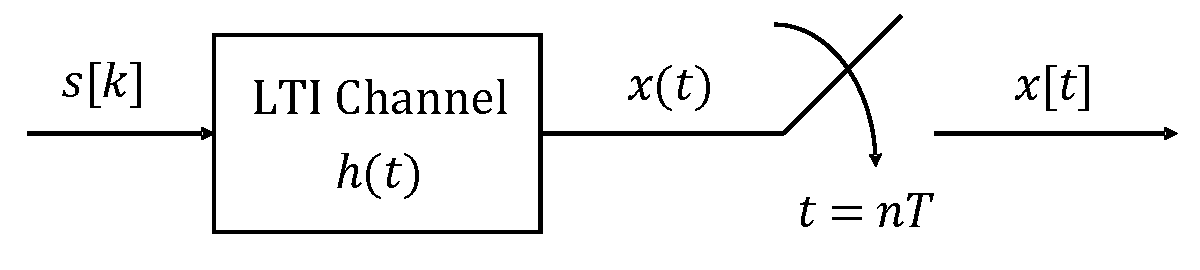
\includegraphics[width=0.8\linewidth]{./figs/bb_system.pdf}
	\caption{Complex baseband equivalent model of a communication system.}
	\label{fig:qamsystem}
\end{figure}
Therefore, the output signal of the overall system can be described as 
\begin{equation}
x[k]=x(kT)=\sum_{i=-\infty}^{\infty} s[i]h(kT-iT+t_0)+n(kT)=\sum_{i=-\infty}^{\infty} h[k]s[k-i]+n[k].
\end{equation}
A non-ideal channel has more than one nonzero component, and thus introduces distortion as the channel output depends on multiple symbols. This is known as inter-symbol interference (ISI), and can severely corrupt the transmitted signal. The goal of equalization is to find a filter $w[k]$ that allows the removal of distorsion. In most real-world scenarios, channels an be described with a finite response of length $L_h$, and in practice equalizers are implemented as an FIR filter of length $L_e\geq L_h$ such that 
\begin{equation}
y[k]=\sum_{m=1}^{L_e} \overline{w}[m]x[k-m] \approx s[k-v],
\end{equation}
with $v$ a constant integer delay, which is acceptable in communication systems. Note that this equation can be written in vector form (disregarding noise) as 
\begin{equation}
y[k]=\bm{w}\herm \bm{x}_k = \bm{w}\herm \mathcal{T}_{L_h}(h)\bm{s}_k, \label{eqn:signalmodel_siso}
\end{equation}
where
\begin{align}
\bm{x}_i&=\begin{bmatrix}x[i]\\ x[i-1]\\ \vdots\\ x[i-L_e+1]\end{bmatrix},\quad \bm{s}_k = \begin{bmatrix}s[i]\\ s[i-1]\\ \vdots\\ s[k-L_h-L_e+1]\end{bmatrix},\quad \bm{w}=\begin{bmatrix}w[1]\\w[2]\\ \vdots\\ w[L_e]\end{bmatrix},\\
\mathcal{T}_{L_h}(h)&=\begin{bmatrix}
h[1]  & h[2]   & \ldots & h[L_h] & 0     & \cdots & 0 \\
0     & h[1]   & h[2]   & \cdots & h[L_h]& \cdots & 0 \\
\vdots& \vdots & \ddots & \ddots &\ddots & \ddots & \vdots\\
0     & 0      & \cdots &  h[1]  & h[2]  & \cdots & h[L_h]
\end{bmatrix} \label{eqn:signalmodeldesc_siso}
\end{align}
are the received signal vector, the transmitted signal vector, the equalizer parameter vector, and the so-called \emph{channel convolution matrix} of size $L_e \times (L_h+L_e-1)$, respectively.

The extension of this model to multiple input and/or multiple output systems is rather straightforward. In the case of single-input multiple-output (SIMO) systems, there are $M$ different LTI channels $h_m[k]$, $m\in{1,\ldots,M}$ with a maximum finite length $L_h$, fed with the same sequence $s[k]$, producing $M$ outputs $x_m[k]$. One filter is provided to each of these outputs, and the system equalizer is the combination of all these filters.  Hence, channel, outputs and equalizers can be arranged as vectors
\begin{align}
\vec{h}[i]=\begin{bmatrix}h_1[i]\\ \vdots\\ h_M[i]\end{bmatrix}\in\mathbb{C}^M,\quad \vec{x}[i]=\begin{bmatrix}x_1[i]\\ \vdots\\ x_M[i]\end{bmatrix}\in\mathbb{C}^M,\quad \vec{w}[i]=\begin{bmatrix}w_1[i]\\ \vdots\\ w_M[i]\end{bmatrix}\in\mathbb{C}^M,
\end{align}
and the whole system can be described as in Eq.(\ref{eqn:signalmodel_siso}) ignoring noise,
\begin{equation}
y[k]=\sum_{m=1}^{L_e} (\vec{w}[m])\herm\vec{x}[k-m]= \bm{w}\herm \bm{x}_k = \bm{w}\herm \mathcal{T}_{L_h}(\vec{h})\bm{s}_k, \label{eqn:signalmodel_simo}
\end{equation}
but redefining these variables as
\begin{align}
\bm{x}_i&=\begin{bmatrix}\vec{x}[i]\\ \vec{x}[i-1]\\ \vdots\\ \vec{x}[i-L_e+1]\end{bmatrix},\quad \bm{s}_k = \begin{bmatrix}s[i]\\ s[i-1]\\ \vdots\\ s[k-L_h-L_e+1]\end{bmatrix},\quad \bm{w}=\begin{bmatrix}\vec{w}[1]\\\vec{w}[2]\\ \vdots\\ \vec{w}[L_e]\end{bmatrix},\\
\mathcal{T}_{L_h}(\vec{h})&=\begin{bmatrix}
\vec{h}[1] & \vec{h}[2] & \ldots     & \vec{h}[L_h] & \vec{0}      & \cdots & \vec{0} \\
\vec{0}    & \vec{h}[1] & \vec{h}[2] & \cdots       & \vec{h}[L_h] & \cdots & \vec{0} \\
\vdots     & \vdots     & \ddots     & \ddots       & \ddots       & \ddots & \vdots  \\
\vec{0}    & \vec{0}    & \cdots     & \vec{h}[1]   & \vec{h}[2]   & \cdots & \vec{h}[L_h]
\end{bmatrix}. \label{eqn:signalmodeldesc_simo}
\end{align}

Multiple-input multiple-output systems follow the same convention, but now there are $L$ sources of data symbols $s_l[k]$. Hence, the LTI channels are now $M\times L$ matrices $\bm{H}[k]$, the outputs and equalizer are vectors $\vec{x}[k],\vec{w}\in\mathbb{C}^M$, and the inputs can be arranged in vector form as $\vec{s}[k]=\big[s_1[k] \ldots s_L[k]\big]\T\in\mathbb{C}^L$, hence  
\begin{equation}
y[k]=\bm{w}\herm \bm{x}_k = \bm{w}\herm \mathcal{T}_{L_h}(\bm{H})\bm{s}_k, \label{eqn:signalmodel_mimo}
\end{equation}
but these signals and channel convolution matrix are now given by
\begin{align}
\bm{x}_i&=\begin{bmatrix}\vec{x}[i]\\ \vec{x}[i-1]\\ \vdots\\ \vec{x}[i-L_e+1]\end{bmatrix},\quad \bm{s}_k = \begin{bmatrix}\vec{s}[i]\\ \vec{s}[i-1]\\ \vdots\\ \vec{s}[k-L_h-L_e+1]\end{bmatrix},\quad \bm{w}=\begin{bmatrix}\vec{w}[1]\\\vec{w}[2]\\ \vdots\\ \vec{w}[L_e]\end{bmatrix},\\
\mathcal{T}_{L_h}(\bm{H})&=\begin{bmatrix}
\bm{H}[1] & \bm{H}[2] & \ldots     & \bm{H}[L_h] & \bm{0}      & \cdots & \bm{0} \\
\bm{0}    & \bm{H}[1] & \bm{H}[2] & \cdots       & \bm{H}[L_h] & \cdots & \bm{0} \\
\vdots     & \vdots     & \ddots     & \ddots       & \ddots       & \ddots & \vdots  \\
\bm{0}    & \bm{0}    & \cdots     & \bm{H}[1]   & \bm{H}[2]   & \cdots & \bm{H}[L_h]
\end{bmatrix}. \label{eqn:signalmodeldesc_mimo}
\end{align}


\subsection{Practical zero-ISI channels}\label{ofdm}
Real-world communication channels are subject to limited bandwidth, channel fading and multipath, and so are afflicted by ISI. However, several modern systems use Orthogonal Frequency Division Multiplexing (OFDM), which is a method that encodes the transmitted signal in multiple carrier frequencies and eliminates ISI. 
A classical OFDM system with $N$ subcarriers uses a $N$-point Discrete Fourier Transform (DFT) in order to remove inter-symbol interference (ISI). A vector $\bm{s}$ containing $N-L_c$ data symbols, also known as a OFDM block, has a cyclic prefix of length $L_c$ added and then is coded before transmission by the DFT matrix $\bm{F}$, with $\bm{FF}\herm=\bm{I}_N$, to finally be transmitted over a distorting mixing channel $\bm{C}\in\mathbb{C}^{N\times N}$. The received signal is given by
\begin{equation}
\bm{\tilde{x}}=\bm{C}\bm{F}\bm{s} + \bm{\tilde{n}},
\end{equation}
where $\bm{\tilde{n}}\in\mathbb{C}^N$ is additive white Gaussian noise (AWGN). The corresponding receiver performs the inverse DFT operation as
\begin{equation}
\bm{x}=\bm{F}\herm\bm{\tilde{x}}=\bm{F}\herm\bm{C}\bm{F}\bm{s} + \bm{F}\herm\bm{\tilde{n}}=\bm{D}\bm{s}+\bm{n},
\end{equation}
where the diagonal matrix $\bm{D}$ is the result of the diagonalization performed over the distorted channel by the DFT matrices, and $\bm{n}$ is AWGN \cite{Ding2009book}. Therefore, the OFDM system has $N$ parallel subchannels, each being a scalar AWGN channel with gain given by the corresponding diagonal element of $\bm{D}$:
\begin{equation}
x_m=D_{mm}s_m+n_m. \label{eqn:ofdm_subchannel}
\end{equation} 

With all subchannels being parallel and independent from each other, the corresponding signals can be processed independently with the same signal model of Eq.~(\ref{eqn:ofdm_subchannel}). Thus, for the sake of notational simplicity, in the following we drop the subchannel notation, and every model below should be understood to apply for all subchannels.

\section{Blind Beamforming}\label{systemModel:beamforming}
\subsection{Blind Signal Recovery with CMA}\label{beamforming}
\begin{figure}
	\centering
	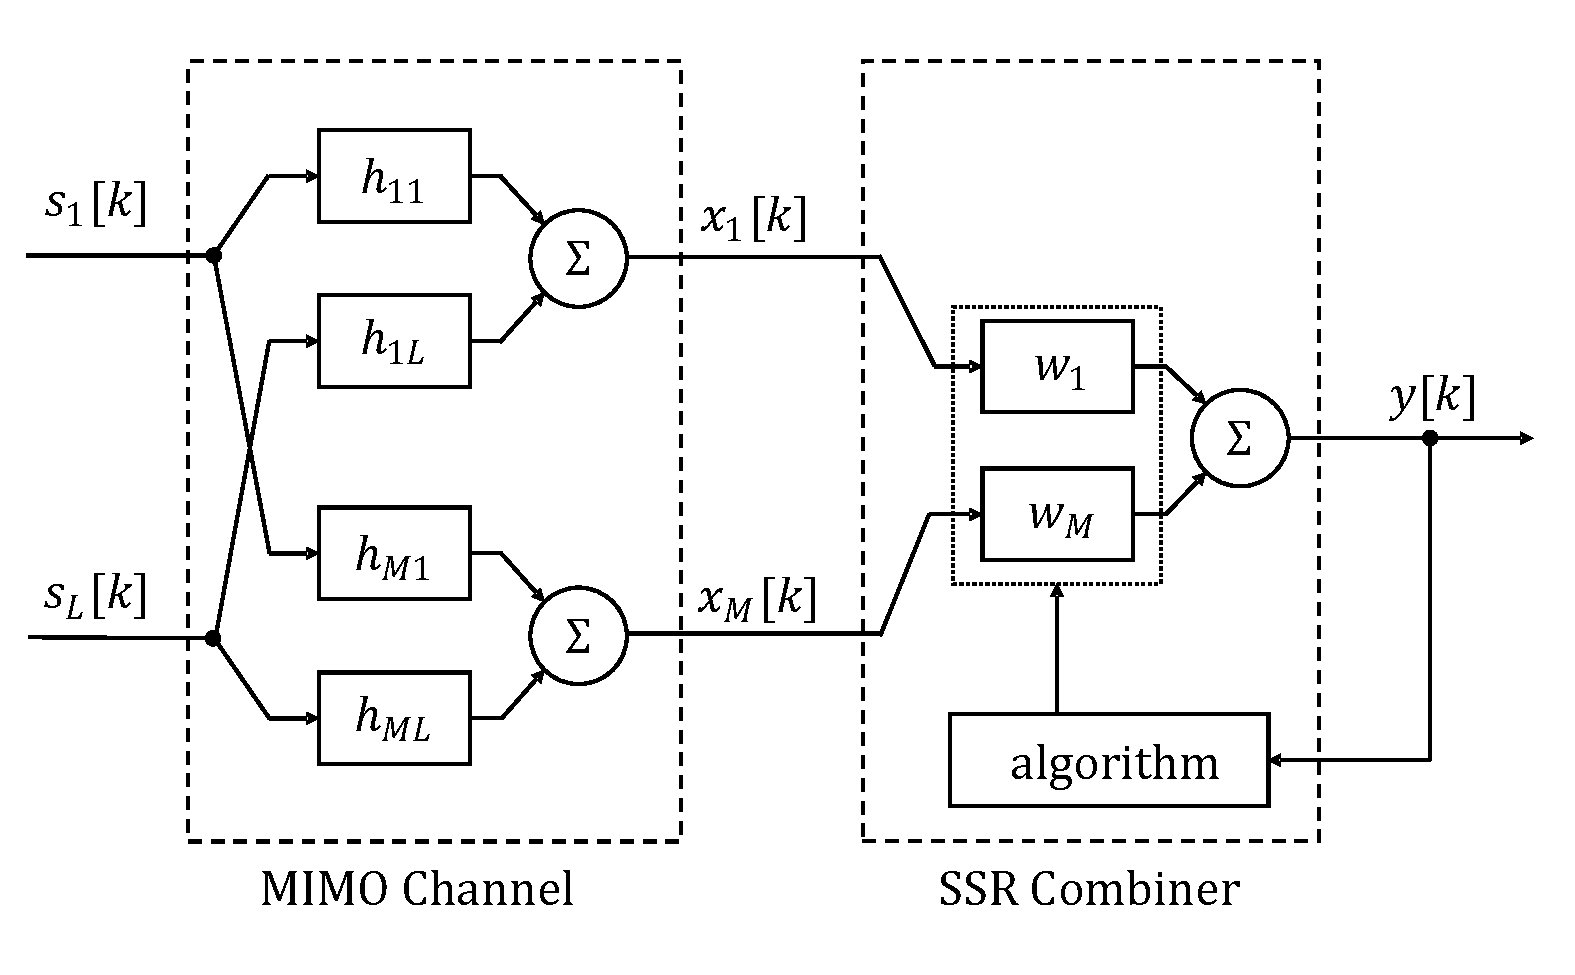
\includegraphics[width=0.9\linewidth]{./figs/ssr_beamforming2.pdf}
	\caption{Blind beamforming. $L$ single-antenna sources are sensed by a receiver with $M$ antennas, which combines them to recover one of those sources with minimal interference.} \label{fig:beamforming}
\end{figure}
Consider the system depicted in Fig.~\ref{fig:beamforming}. There are $L$ single-antenna sources that transmit independent symbols, each represented by $s_l[k]\in\mathbb{C}$ at time $k\in\{1,\ldots,K\}$ and source $l\in\{1,\ldots,L\}$. The receiver has $M$ antennas, each of one receiving a combination of all sources via a zero-ISI flat-fading MIMO wireless channel $\bm{H}\in\mathbb{C}^{M\times L}$ plus AWGN $\bm{w}_k\in\mathbb{C}^M$. Using the model for MIMO systems introduced in Eq.(\ref{eqn:signalmodel_mimo}), the received signal vector at time $k$ is
\begin{equation}
\bm{x}_k=\bm{H}\bm{s}_k+\bm{n}_k \label{eqn:rxsignal}
\end{equation}
where the channel $\bm{H}$ has full column rank. We are interested in finding $\bm{\hat{w}}\in\mathbb{C}^M$ such that it is possible to recover one of the sources with minimal interference, that is, 
\begin{equation}
y[k]=\hat{\bm{w}}\herm\bm{x}_k\approx{s}_l[k],\quad\text{for some}\,\,l\in\{1,\ldots,L\} \label{eqn:combineroutput}
\end{equation}
with no more information that the received signal samples, i.e., no other property of the transmitted signal is known. In the following, this will be denoted as the single source recovery problem.

As described in \cite{Godard1980cma}, the constant modulus algorithm provides a means to adaptively find the optimum combiner $\bm{\hat{w}}$ that solves 
\begin{equation}
\text{minimize}\quad\frac{1}{K}\sum_{k=1}^K\Big(|y_k|^2-R_2\Big)^2 \label{eqn:cma_orig}
\end{equation}
where, assuming that all signals have the same statistics, 
\begin{equation}
R_2 = \frac{E\{|s_l[k]|^4\}}{E\{|s_l[k]|^2\}}. \label{eqn:r2_orig}
\end{equation}

Knowing that $|y[k]|^2=|\bm{w}\herm\bm{x}_k|^2$, we can rewrite $\mathcal{P}$ as
\begin{eqnarray}%\bm{w}_*=\argmin_{\bm{w}\in\mathcal{C}^M}
\mathcal{P}:\,\,\min_{\bm{w}\in\mathbb{C}^M}\quad f(\bm{w})=\displaystyle{\frac{1}{K}\sum_{k=1}^K\Big(|\bm{w}\herm\bm{x}_k|^2-R_2\Big)^2} \label{eqn:cma}
\end{eqnarray}
which is a biquadratic smooth real-valued function of $\bm{w}$, and as such is non-convex. Also note that the problem is phase-invariant, as any rotation of $\bm{w}$ is also a solution, i.e., $\bm{w}'=\alpha\bm{w}$ with $\alpha\in\mathbb{C},|\alpha|=1$ also minimizes $\mathcal{P}$. 

Despite its name, CMA can be applied to iid. signals using QAM constellations of arbitrary size and varying magnitude, as long as the contellations satisfy some symmetry and higher-order moments restrictions \cite{Ding2000}.
Though the selection of $R_2$ requires the distribution information of the transmitted signals $\bm{s}_k$, it is known that one can select a positive constant value (usually set equal to 1), and the CMA algorithm will yield a combiner that recovers a scaled version of the QAM signal, without changing the constellation shape. 


\subsection{Blind Multiple Signal Recovery using CMA}

%{\bf Again we need to talk about Grant Free Access setup here:
%}
%With the expansion of massive IoT, the question whether is possible to recover more than one source is evident. 
In the context of massive IoT, however, it is far more interesting to be able to recover more than one source under the same conditions as before, that is, no pilots or preambles, no previous knowledge of the transmitted signals, and no channel information. 
This can be addressed by obtaining $J\leq L$ optimal combiners $\hat{\bm{w}}_j$ in the receiver, each different from each other and tuned to different signals, that is,
\begin{equation}
\bm{y}[k]=\begin{bmatrix}
y_1[k]\\
\vdots\\
y_J[k]\herm\\
\end{bmatrix}=\begin{bmatrix}
\hat{\bm{w}}_1\\
\vdots\\
\hat{\bm{w}}_J\herm\\
\end{bmatrix}
\bm{x}_k\approx
\begin{bmatrix}
{s}_{l_1}[k]\\
\vdots\\
{s}_{l_J}[k]\end{bmatrix},\quad\text{with}\,\,
l_j\in\{1,\ldots,L\},\quad j\in\{1,\ldots,J\},
\end{equation}
where the recovery has no particular order respect to the assigned indexing of the sources. Fig.~\ref{fig:beamformingMSR} shows this extension of the original blind beamforming problem, which will be denoted as multiple source recovery (MSR).
\begin{figure}
	\centering
	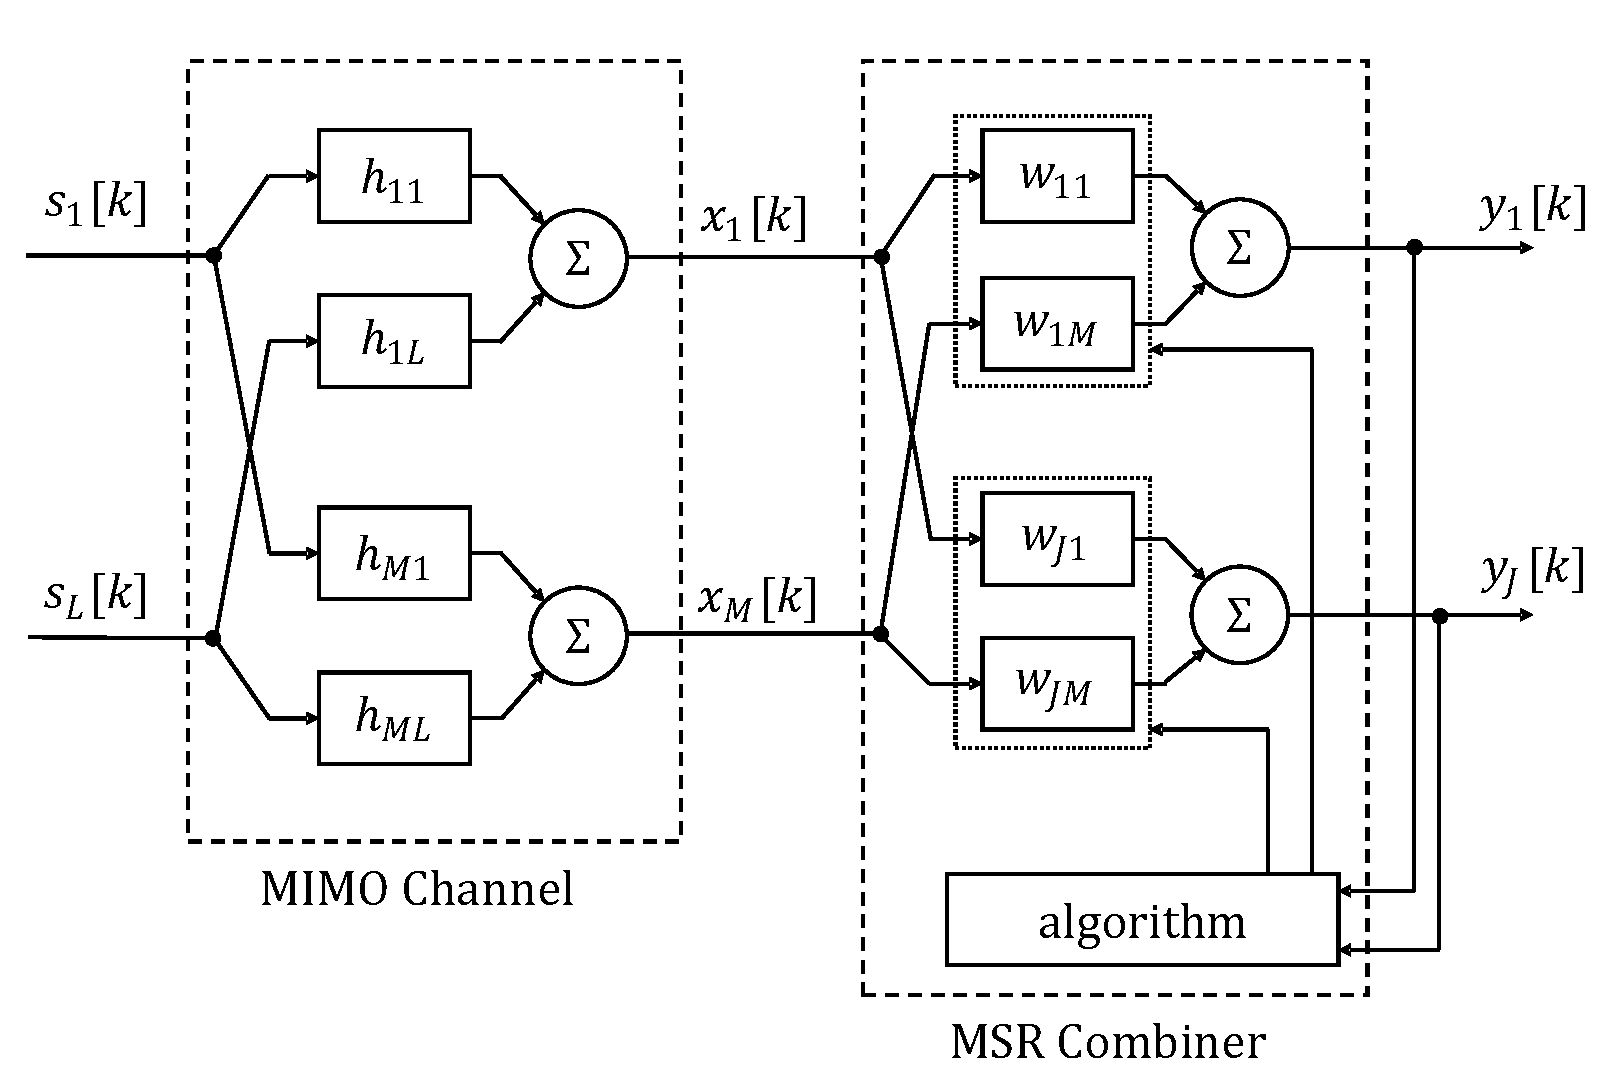
\includegraphics[width=0.9\linewidth]{./figs/msr_beamforming2.pdf}
	\caption{Blind beamforming with multiple source recovery. The receiver now has $J$ combiners to recover $J$ of the $L$ sources with minimal interference.} \label{fig:beamformingMSR}
\end{figure}

Now, considering the multiple blind equalizer from Fig.~\ref{fig:beamformingMSR}, it is viable to minimize the blind beamforming problem for each individual output, obtaining corresponding combiners that will restore one of the sources. However, with no other considerations included, it is very likely that all combiners will restore the same source signal, possibly with different phases and even with different delays \cite{Ding2000}. Therefore, when considering multiple signal recovery, problem $\mathcal{P}$ needs to be modified in order to force the different combiners $\bm{w}_j,\,j\in\{1,\ldots,J\}$ to recover different source signals. Given that the different sources are independent, this is equivalent to force statistical uncorrelatedness of the signals. For the case of complex outputs $y_{j_1},y_{j_2}$, their covariance is given by:
\begin{align}
\mathrm{Cov}\{y_{j_1},y_{j_2}\}
&=\mathbb{E}\{y_{j_1}y_{j_2}^*\}
=\mathbb{E}\{ \bm{w}_{j_1}\herm\bm{x_k}(\bm{w}_{j_2}\herm\bm{x_k})^*\}
%\nonumber\\&
=\mathbb{E}\{ \bm{w}_{j_1}\herm\bm{X}_k\bm{w}_{j_2}\}=\bm{w}_{j_1}\herm\mathbb{E}\{\bm{X}\}\bm{w}_{j_2}.
\end{align}

Thus, we propose to regularize the CMA cost function with the magnitude squared of the pairwise covariances of the outputs, to obtain a smooth real-valued cost function. Thus, the modified CMA cost function with multiple signal recovery consists on the sum of the base CMA function for each combiner, adding the magnitude squared of each pairwise covariance: 
\begin{equation}
\mathcal{P}_J:\,\text{min}\,\, g(\bm{w}_1,\ldots,\bm{w}_J)=\sum_{j=1}^Jf(\bm{w}_j) +\gamma_0\sum_{j_1\neq j_2}^J\big|\bm{w}_{j_1}\mathbb{E}\{\bm{X}\}\bm{w}_{j_2}\big|^2 \label{eqn:cma_msr}
\end{equation}
where $\gamma_0>0$, as the magnitude squared of the covariances is always positive.  
Note that this is a reduced version of the regularization proposed in \cite{Chen1991crimno,Li1998adaptivemimocma}, where the authors propose the use of joint cumulants for source separation. The joint cumulants also consider the potential correlatedness of delayed versions of the combiner outputs, but in the presented case of beamforming the channels have no ISI, and the information from different delays of the outputs is not necessary. This cost function is also presented in \cite{Ikhlef2007simplifiedmimocma}, although they only use the real part of the equalized signal in their formulation.

\section{Convergence guarantees}
The global convergence properties of CMA for PAM and QAM modulations in noiseless scenarios are well known \cite[Chapters 4, 7]{Ding2000}.  The case of SIMO-CMA blind equalizers, also known as fractionally-spaced CMA or CMA-FSE (when applied to blind equalization scenarios), correspond to the case of recovering the transmitted signal via multiple antennas (for blind beamforming) or an oversampled equalizer (for blind equalization). The CMA-FSE equalizer has guaranteed global convergence as long as the subchannels have no common zeros, when using an equalizer with memory length larger than the order of the channel \cite{LiDing1994cmaglobalconvergencefse}.

MIMO-CMA equalizers are an extension of CMA-FSE, where multiple sources are transmitting independent sources, and we adaptively find an equalizer that recovers one signal with minimal multi-user interference and minimum ISI \cite{Mayrargue1994mimocma,Li1998adaptivemimocma}. For such a channel, the channel convolution matrix $\mathcal{T}_{L_h}(\bm{H})$ is described in Eq.(\ref{eqn:signalmodeldesc_mimo}), which is formed by the different MIMO-channel delays $\bm{H}[m]$. Here, global convergence requires the channel convolution matrix to have full column rank and vector equalizers with memory length larger than the order of the channels.
 
The presented CMA-based single source recovery corresponds to a particular case of the MIMO-CMA blind equalizer, where the channel has no ISI and we only aim to remove multi-user interference, thanks to OFDM. Thus, in this case, the length of the channel is $L_h=1$ and the channel convolution matrix $\mathcal{T}_{L_h}(\bm{H})$ is equal to the channel matrix $\bm{H}$, and thus we only need the latter with full column rank to have guaranteed global convergence in noiseless scenarios, regardless of initial conditions. Multiple source recovery also acts as a special case of the multiple source recovery scheme presented \cite{Li1998adaptivemimocma} with zero-ISI subchannels, and therefore global convergence is also guaranteed under similar conditions. Hence, in the following we will always assume that the channel matrix $\bm{H}$ has full-column rank.

% Succinctly, for a noiseless MIMO system with $M$ receiving antennas and a maximum channel order of $L_h$, any MIMO-CMA linear blind equalizer of order $L_e\geq ML_h-1$ can achieve global convergence to capture one of the user signals, regardless of initial setting. The considered beamforming scenarios are not subject to ISI, thus the maximum order of the MIMO channel is $L_h=0$ (as every subchannel consists only on a complex scalar gain), thus we only need an equalizer of order $L_e\geq -1$. Thanks to OFDM, thus, there is no requirement on the equalizer order to attain global convergence.

When considering noisy transmissions, it is well known that the effect of the noise is the addition of local minima to the cost function \cite{Ding2000}. For gradient-descent based methods, this usually implies a careful selection of the stepsize (usually based in trial and error), and even then there is no guarantee that the optimization method will yield a global minimizer. Thus, the study of new approaches and results that can provide better guarantees in the selection of the stepsize are of special interest.

Second-order optimization methods, on the other hand, can deal with saddle points that gradient descent cannot distinguish from local minima, but suffer when solutions are not unique, such as the case with CMA \cite{Kreutz2008trustregionscma}, requiring regularization or other techniques in order to provide convergence guarantees. 